
\chapter{\'Etude du corpus de son \textit{ambiance}}
\label{chap:ambiance}
Dans ce chapitre, on étudie le comportement des différentes versions de la NMF, présentées dans le chapitre \ref{chap:nmf},  avec le premier corpus élémentaire \textit{Ambiance}. 

Nous ferons dans un premier temps un rappel du corpus, des méthodes choisies et une présentation de la méthode de référence (ou \textit{baseline} en anglais). Puis les étapes menant à l'apprentissage du dictionnaire sont détaillées. Enfin les résultats des calculs menés sur le corpus sont présentés.

Le corpus de scènes est composé, pour rappel, de 6 sous-corpus : \textit{alert}, \textit{animaux}, \textit{climat}, \textit{humain}, \textit{transport}, \textit{mécanique}. Dans chaque sous-corpus, un signal \textit{trafic}, qui considère le bruit de fond routier ainsi que les évènements sonore \textit{passages de voitures}, est calibré par rapport au niveau sonore de classe de sons \textit{interférante} qui est composé des autres signaux sonores : 

\begin{equation}
TIR = L_{eq,trafic} - L_{eq,interferant}
\end{equation}

avec $TIR \in \lbrace -12,~-6,~0,~6,~12 \rbrace$. Ce corpus permet de tester les performances de la NMF et son comportement face à de tel mixtures sonores. Dans un premier temps, la composition du dictionnaire est décrite. Puis un résumé des facteurs expérimentaux impliqués est présenté.
En tout, 750 scènes d'une durée individuelle de 30 secondes (pour une durée totale de 6h20).
Pour chaque scène, le niveau sonore global du trafic estimé par la baseline, $\tilde{L}_{eq,trafic}$. Pour chaque sous-corpus et valeur du TIR, les 25 niveaux estimés sont comparés à leur niveau sonore exacte, $L_{eq,trafic}$ au travers de METRIQUE.
Cette métrique sera alors moyenné sur l'ensemble des sous-classes de sons par TIR : 

\begin{equation}
E = \frac{\sum_{i = 1}^6 METRIQUE_{i}}{6}
\end{equation}

Cette indicateur renseigne alors les performances de l'estimateur sur l'ensemble des sous-classes par TIR. Il est également possible de calculer cette indicateur sur l'ensemble des sous-classes et de TIR pour connaitre la combinaison de l'estimateur qui donne l'erreur la plus faible sur l'intégralité du corpus : 

\begin{equation}
E = \frac{\sum_{i = 1}^6 \sum_{j = 1}^5 METRIQUE_{i,j}}{6 \times 5}
\end{equation}



\section{Constitution du dictionnaire}
Dans un premier temps, le dictionnaire $\mathbf{W}$ est construit, à partir du corpus de référence, composé des fichiers audio des passages des voitures enregistrés des voitures Renault Scénic et Dacia Sandero sur la piste d'essais. Ces 53 échantillons audio issus des enregistrements ne sont pas ceux utilisés dans la création des scènes sonores afin d'éviter tout problème de sur-apprentissage.

\begin{figure}[hbtp]
\centering
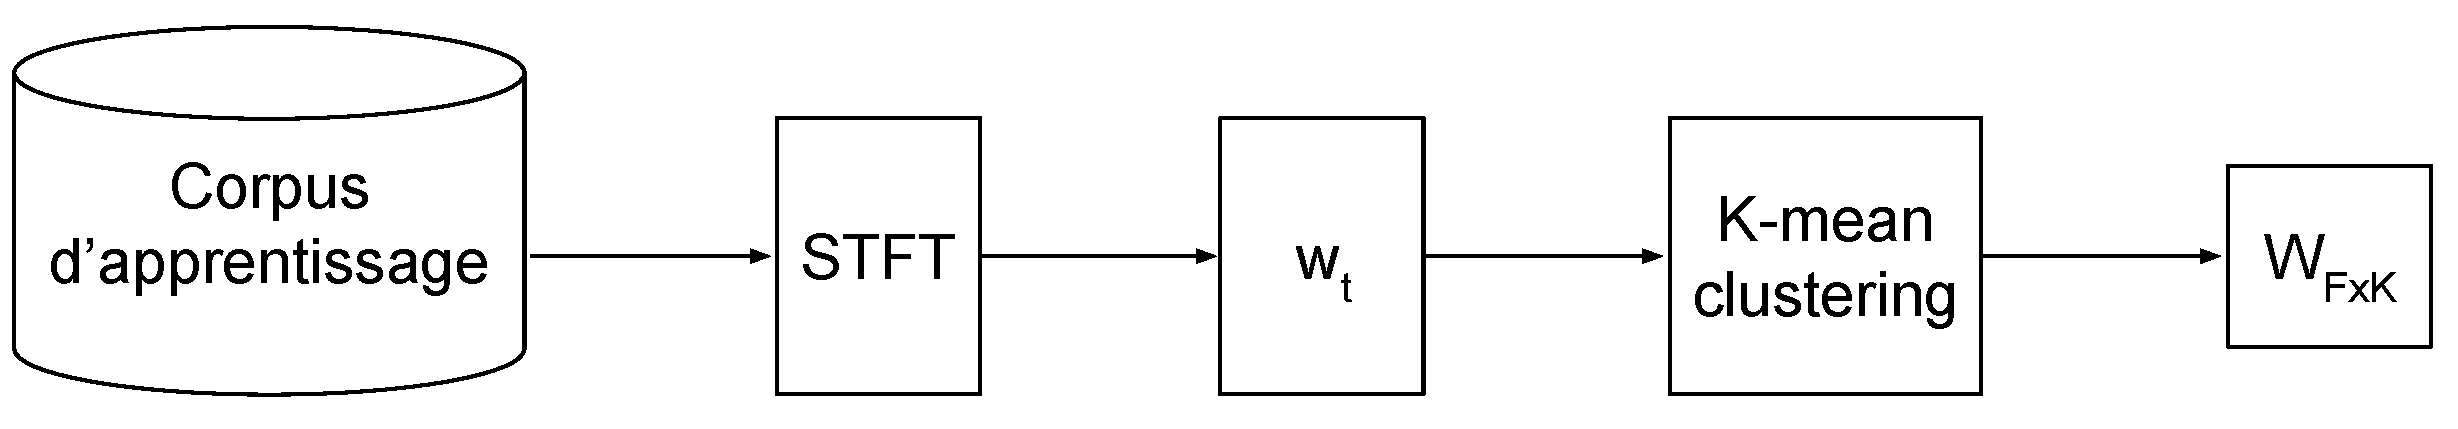
\includegraphics[width=.9\linewidth]{./figures/NMF/creation_dictionaire.pdf}
\caption{Diagramme en blocs de la création du dictionnaire}
\label{fig:creation_W}
\end{figure}


La constitution du dictionnaire est réalisée en trois étapes, résumée dans le diagramme en bloc en Figure \ref{fig:creation_W} : 
\begin{itemize}
\item chaque fichier audio est représenté au travers d'un spectrogramme, obtenu par une STFT (nombre de point $w = 2^{12}$ avec 50 $\%$ de recouvrement). Cette première étape permet de représenter chaque échantillon audio, de durée différente, avec le même nombre de point en fréquences.
\item Chaque spectrogramme est ensuite découpé en plusieurs trames de largeur $w_t \in \lbrace 0,5~ 1~ 2~\rbrace$ seconde. Dans chaque trame la valeur efficace (ou valeur \textit{rms} en anglais) sur chaque trame fréquentiel est calculé. Cet étape a pour but de décrire en différentes formes les 53 échantillons audio. Pour $w_t = 0,5$, on obtient une description plus fine que dans le cas où $w_t = 2$. Les détails de cette étape est décrit en Figure \ref{fig:decoupe_W}.
\item Enfin, l'opération précédente générant un grand nombre de fichier (2218 pour $w_t$ = 0,5 s, 505 éléments pour $w_t$ = 2 s), un algorithme de clustering $K$-mean est appliqué en vue de réduire ce nombre, d'éviter la présence d'informations redondates et de fixer le nombre d'éléments à $K = \lbrace 25,~50,~100,~200 \rbrace$. Les $K$ clusters déterminés sont alors les éléments qui composent le dictionnaire $\mathbf{W}$.
\end{itemize}

En plus de ces étapes, on ajoute un cas où la valeur \textit{rms} est calculé sur l'ensemble des spectrogrammes ($w_t = all$). En cela, des 53 fichiers audio, 53 spectres sont générés. Ces 53 spectres sont également soumis à l'algorithme de clustering mais avec cette fois, $K \in \lbrace 25 50 \rbrace$.

En tout, c'est donc 14 versions de dictionnaire qui sont réalisées ($4\times 3 + 1 \times 2$).

\begin{figure}[hbtp]
\centering
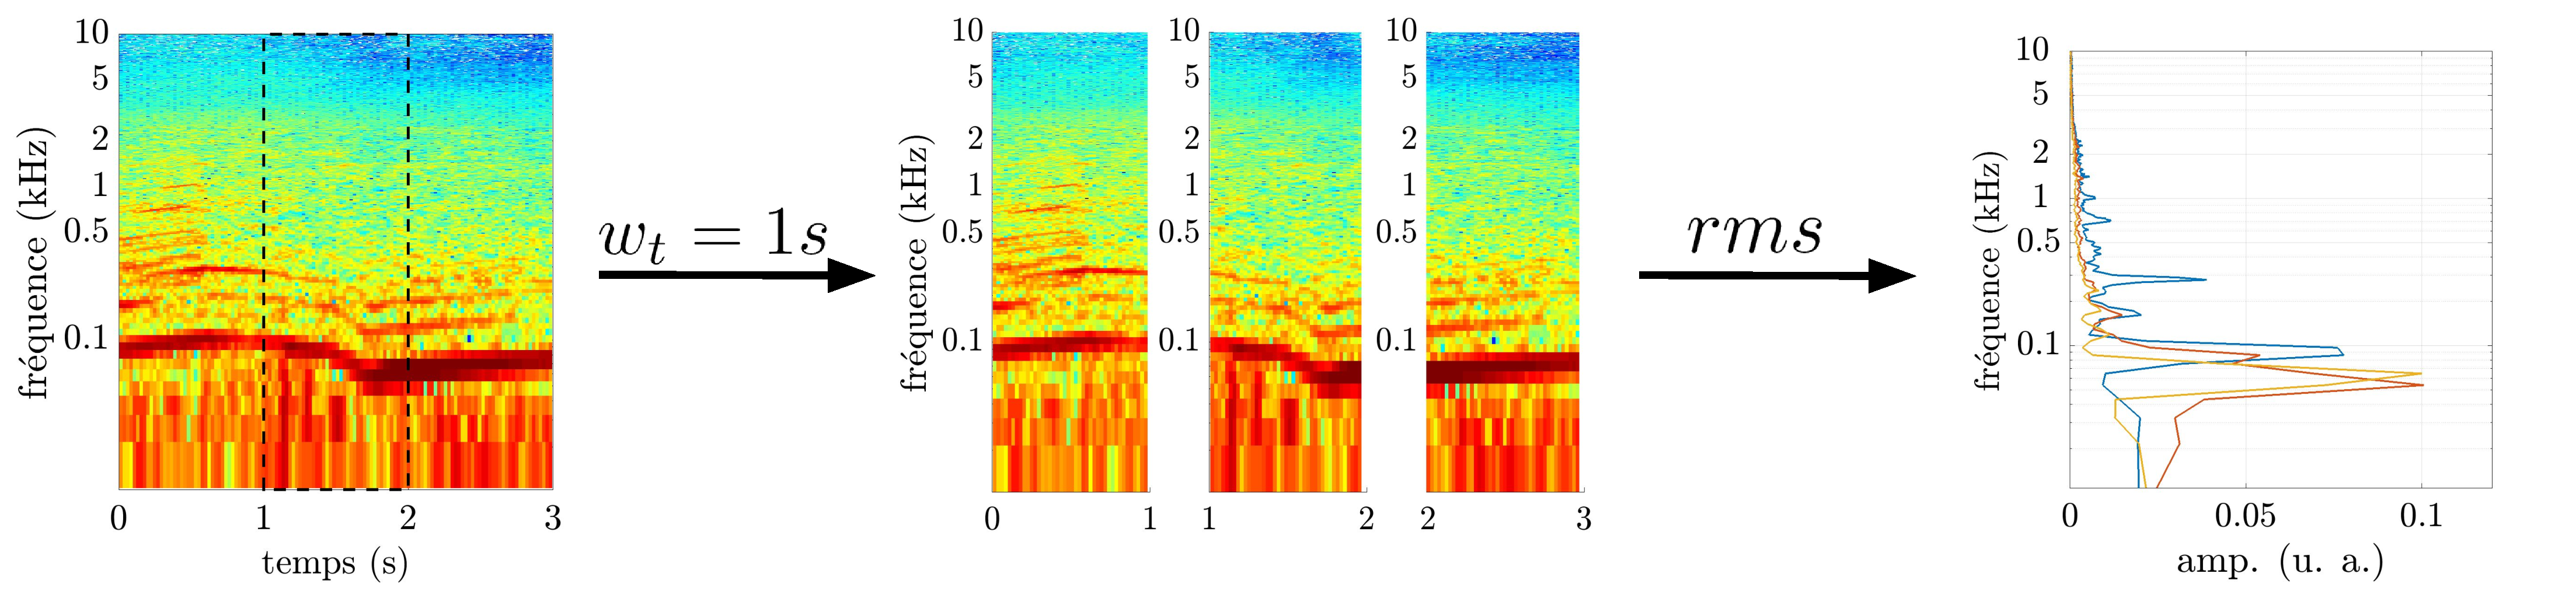
\includegraphics[width=.9\linewidth]{./figures/NMF/dictionaire_frame_FR.pdf} 
\caption{Création des éléments sur un extrait de 3 secondes du passage d'une voiture pour une largeur de la trame temporelle $w_t$ de 1 seconde. À gauche le spectrogramme du signal audio avec, en pointillés, une fenêtre de découpe de largeur $w_t$. Le signal est ainsi découpé en trois parties dont les valeurs \textit{rms} sont ensuite calculés. }
\label{fig:decoupe_W}
\end{figure}

\section{Résumé des facteurs expérimentaux}

À partir de ces versions de dictionnaire, la NMF supervisée (NMF-SUP), semi-supervisée (NMF-SS) et Initialisée-seuillée (NMF IS) sont calculés. Pour chacune, 3 $\beta$-divergences sont invoqués : la distance Euclidienne ($\beta = 2$), équation \ref{}, la divergence de Kullback-Leibler ($\beta = 1$), équation \ref{}, et la divergence d'Itakura-Saïto ($\beta = 0$), equation \ref{}.
\'Egalement, une représentation en bande tiers-d'octave a été choisie pour $\mathbf{W}$ et $\mathbf{V}$. Cette représentation a plusieurs intérets : 

\begin{itemize}
\item par son échelle logarithmique, elle permet de mieux décomposer les basses fréquences que les hautes fréquences. On permet alors de mieux focaliser la reconstruction du signal vers les bandes de fréquences d'intérêts.
\item Cette représentation est également couramment utilisée dans le domaine de l'acoustique urbaine et environnementale, à la différence des MFCC. En vue des applications prévue de ces outils (amélioration de la cartographie, estimation des sources sonores urbaines), c'est une représentation plus adaptée.
\item enfin, le nombre de bande étant réduites ($F = 29$), la manipulation des matrices est plus rapide qu'avec des bandes fines et donc permet un gain en temps de calculs.
\end{itemize}

Les 14 versions du dictionnaires sont alors testées pour les 3 NMF. Dans le cas de la NMF-SS, ces dictionnaires sont associés au dictionnaire mobile $\mathbf{W_r}$ dont la dimension est fixé à 2 ($J = 2$).
Dans le cas de la NMF IS, ce dictionnaire correspond au dictionnaire initial $W_0$ qui sera ensuite mis à jours. De plus, de nombreuses combinaisons sont réalisées selon  : 
\begin{itemize}
\item la représentation de la distance (linéaire ou bien exprimé au travers d'une fonction sigmoïde),
\item le type de seuillage (dur ou \textit{firm}),
\item les valeurs des différents seuils ($t_h$ et $t_{f,1/2}$). Des études préliminaires ont permis de réduire les valeurs limites de ces seuils à $t_h \in \lbrace \rbrace$, $t_{f,1} \in \lbrace \rbrace$ et $t_{f,2} \in \lbrace \rbrace$, chacune étant défini avec un pas de 0,01.
\end{itemize}

L'ensemble des paramètres est résumé dans le Tableau \ref{tab:experimental_factorsNMF_ambiance}. Le nombre de combinaison des modalités est alors de 
Enfin XX itérations sont réalisées. 

Les calculs sont réalisés sous le logiciel Matlab, avec l'aide de l'outil expLanes\footnote{\url{http://mathieulagrange.github.io/expLanes/}} qui permet la réalisation d'expériences numérique, de gérer la distribution des nombreux facteurs expérimentaux et leur modalités et de collecter les nombreux résultats générés.

\begin{table*}[t]
\centering
\caption{Facteurs expérimentaux et leur modalité utilisé pour le corpus \textit{Ambiance}.}
\begin{tabularx}{17.5cm}{L{3cm}@{}C{12cm}@{}C{2cm}@{}}
	\hline
    \textbf{\begin{tabular}[c]{@{}l@{}}facteur \\ expérimentaux \end{tabular}} & \textbf{modalités} & \begin{tabular}[c]{@{}C{2cm}@{}}\textbf{nombre de}\\ \textbf{modalité}\end{tabular}\\ \toprule
\end{tabularx}

\begin{tabularx}{17.5cm}{L{2.8cm}@{}@{}C{2cm}@{}@{}C{2cm}@{}@{}C{2cm}@{}@{}C{2cm}@{}@{}C{2cm}@{}@{}C{2.2cm}@{}C{2cm}}
\rowcolor[HTML]{C0C0C0}
   $\mathbf{f_c}$ (kHz) & alerte & animaux & climat &  humain & transport & mécanique & 6\\
\end{tabularx}

\begin{tabularx}{17.5cm}{L{3cm}@{}C{3cm}@{}@{}C{3cm}@{}@{}C{3cm}@{}@{}C{3cm}@{}C{2cm}@{}}
  \textbf{method} & filtre passe bas & NMF SUP & NMF SEM & NMF IS & 4\\
\end{tabularx}

\begin{tabularx}{17.5cm}{L{3cm}@{}@{}C{2cm}@{}@{}C{2cm}@{}@{}C{2cm}@{}@{}C{2cm}@{}@{}C{2cm}@{}@{}C{2cm}@{}C{2cm}@{}}
\rowcolor[HTML]{C0C0C0}
   $\mathbf{f_c}$ (kHz) & 0.5 & 1 & 2 &  5 & 10 & 20 & 6\\
\end{tabularx}

\begin{tabularx}{17.5cm}{L{3cm}@{}C{3cm}@{}@{}C{3cm}@{}@{}C{3cm}@{}@{}C{3cm}@{}C{2cm}@{}}
    $\mathbf{w_t}$ (s)& 0.5 & 1 & 2 & \textit{all} & 4\\
\end{tabularx}

\begin{tabularx}{17.5cm}{L{3cm}@{}C{3cm}@{}@{}C{3cm}@{}@{}C{3cm}@{}@{}C{3cm}@{}C{2cm}@{}}
	\rowcolor[HTML]{C0C0C0}
    $\mathbf{K}$ & 25 & 50 & 100 & 200 & 4\\
\end{tabularx}

\begin{tabularx}{17.5cm}{L{3cm}@{}C{4cm}@{}@{}C{4cm}@{}@{}C{4cm}@{}C{2cm}@{}}
   $\mathbf{\beta}$ & 0 & 1 & 2 & 3\\
\end{tabularx}

\begin{tabularx}{17.5cm}{L{3cm}@{}C{6cm}@{}@{}C{6cm}@{}C{2cm}@{}}
	\rowcolor[HTML]{C0C0C0}
   représentation & linéaire & sigmoïde & 2\\
\end{tabularx}

\begin{tabularx}{17.5cm}{L{3cm}@{}C{12cm}@{}C{2cm}@{}}
	seuillage dur $\mathbf{t_h}$ & de 0.30 à 0.60 avec un pas de 0.01 & 31\\
\end{tabularx}

\begin{tabularx}{17.5cm}{L{3cm}@{}C{12cm}@{}C{2cm}@{}}
	\rowcolor[HTML]{C0C0C0}
   seuillage firm $\mathbf{t_{f,1}}$ & de 0.30 à 0.60 avec un pas de 0.01 & 31\\
\end{tabularx}

\begin{tabularx}{17.5cm}{L{3cm}@{}C{12cm}@{}C{2cm}@{}}
   seuillage firm $\mathbf{t_{f,2}}$ & de 0.30 à 0.60 avec un pas de 0.01 & 31\\
   \bottomrule
\end{tabularx}

\label{tab:experimental_factorsNMF_ambiance}
\end{table*}

\section{Résultats}


\subsection{Performance de l'estimateur \textit{baseline}}

Les résultats issus de l'estimateur baseline sont d'abord présentés. Dans un premier temps, on résumé dans le Tableau les erreurs moyennes émises pour chaque filtre sur l'ensemble du corpus. Les erreurs moyennées sur l'ensemble des sous-corpus par TIR est également résumés. 

\begin{table}[]
\centering
\caption{Erreur XXX de l'estimateur \textit{baseline} selon $f_c$ sur l'ensemble du corpus \textit{Ambiance} et pour chaque TIR}
\label{tab:resuls_ambiance_filtre}
\resizebox{\textwidth}{!}{%
\begin{tabular}{lcccccc}
$f_c$ (Hz) & MAE & -12 & -6 & 0 & 6 & 12 \\ \toprule
100 &  &  &  &  &  &  \\
\rowcolor[HTML]{C0C0C0}
250 &  &  &  &  &  &  \\
500 &  &  &  &  &  &  \\
\rowcolor[HTML]{C0C0C0}
1k &  &  &  &  &  &  \\
2k &  &  &  &  &  &  \\
\rowcolor[HTML]{C0C0C0}
5k &  &  &  &  &  &  \\
10k &  &  &  &  &  &  \\
\rowcolor[HTML]{C0C0C0}
20k &  &  &  &  &  & \\ \bottomrule
\end{tabular}}
\end{table}


\subsection{Résultats de la NMF}

\subsection{Résultats de la NMF-SUP et NMF-SS}

\subsection{Résultats de la NMF-IS}


\begin{itemize}


\item résultats
\begin{itemize}
\item mae générale (filtre VV, supervisé, semi-supervisé, seuillé VV)
\item mae pour chaque TIR et chaque ambiance (filtre VV, supervisé, semi-supervisé, seuillé VV)
\item allure des courbes Lp,1s pour TIR -12 et 12 (supervisé, semi-supervisé, seuillé) dans deux cas extrêmes, y'a des fois ou ça marche moins notamment avec la météo mais ça c'est moins grave (on a des capteurs, on peut les mettre à part, à voir si ce n'est que l'orage)
\item fonction cost (supervisé, semi-supervisé, seuillé)
\item allure des 2 éléments dans Wr
\item distance $w_0$ et $w$
\end{itemize}
\end{itemize}


\begin{table}[h]
\centering
\begin{tabular}{L{5cm} L{5cm}}

\multicolumn{1}{c}{\textbf{paramètre}} & \multicolumn{1}{c}{\textbf{valeurs}} \\ \hline
\textbf{classe de son} & voiture, voiture+oiseaux, toutes les classes \\ \hline
\rowcolor[HTML]{C0C0C0}
\textbf{pas temporel} & 0, 0.5, 1.0 \\ \hline
\textbf{nombre $K$} & 25, 50, 100 \\ \hline
\rowcolor[HTML]{C0C0C0}
\textbf{méthode de réduction} & kmeans, kmeans-medoïd, aléatoire \\ \hline
\end{tabular}
\caption{Valeur des paramètres choisis pour l'élaboration du dictionnaire}
\label{tab:valeur_dictionary}
\end{table}

En tout, 81 différentes versions du dictionnaire sont élaborées.

\subsection{Estimation des niveaux sonores}
L'éatpe suivante consiste à déterminer le niveau sonore du trafic. Deux méthodes sont donc utilisées. Cette estimation se fait à l'aide de la NMF et de ces différentes versions proposés. Pour chacune, le choix de la divergence ($\beta$) ou bien encore les différentes pondérations prennent plusieurs valeurs. La méthode NMF et ces différentes version sont sont comparé à une méthode simple de filtrage passe-bas. Comme l'énergie spectrale du trafic se situe dans les basses fréquences ($\approx \left[0-5000 \right]$ Hz), cette méthode assimile que la partie située dans la bande passante correspond au trafic routier. Cette seconde méthode permet également de comparer les performances de la NMF face à une autre méthode.

La encore plusieurs paramètres interviennent :
\begin{itemize}
\item méthode employée, la NMF ou le filtrage
\item la fréquence de coupure $f_c$
\item la divergence choisie
\item le type de NMF
\item la pondération de la parcimonie
\item la pondération de la \textit{smoothness}
\item l'application de la contrainte sur les éléments du dictionnaire, cette contrainte peut être appliqué sur l'ensemble des éléments du dictionnaire mais peut être appliqué sur les éléments \textit{trafic} seulement,
\item le nombre d'élément $J$ dans $W_r$,
\item la pondération de la contrainte sur $W_r$,
\item le domaine spectrale, le dictionnaire peut être décrit avec une échelle fréquentielle linéaire ou bien par une échelle logarithmique en mel.
\end{itemize}

\begin{table}[h]
\centering
\begin{tabular}{L{5cm} L{5cm}}
\multicolumn{1}{c}{\textbf{paramètre}} & \multicolumn{1}{c}{\textbf{valeurs}} \\ \hline
\textbf{estimateur} & filtrage passe-bas, NMF \\ \hline
\rowcolor[HTML]{C0C0C0}
\textbf{type de NMF} & supervisée, semi-supervisée \\ \hline
\textbf{fréquence $f_c$ (kHz)} & 0.5, 1, 2, 5, 10, 20 \\ \hline
\rowcolor[HTML]{C0C0C0}
\textbf{corpus} & voiture, ambiance, grafic \\ \hline
\textbf{TPR} & -12, -6, 0, 6, 12 \\ \hline
\rowcolor[HTML]{C0C0C0}
\textbf{$\beta$} & 0, 1, 2 \\ \hline
\textbf{$\alpha_{sp}$} & 0, 0.1, 0.5 \\ \hline
\rowcolor[HTML]{C0C0C0}
\textbf{$\alpha_{sm}$} & 0, 1, 5, 10 \\ \hline
\textbf{application $\alpha_{sm}$} & trafic, toutes les classes \\ \hline
\rowcolor[HTML]{C0C0C0}
\textbf{Nombre J} & 2, 3 \\ \hline
\textbf{$\beta_{ss}$} & 1, 2
\end{tabular}
\caption{Valeurs des différents paramètres utilisés dans l'estimation du niveau sonore, les valeurs des pondérations de $\alpha_{ss}$ font l'objet d'une partie en elles seules (voir partie BLABLA).}
\label{tab:valeur_estimation}
\end{table}

Le nombre de combinaison de paramètres dans cette deuxième étape est alors important (plus de 15000 combinaisons possible) auquel s'ajoute les 81 versions du dictionnaire.



%\end{document}
